\chapter{Prototype -- Development and Implementation\label{cha:prototype}}
%5020
This chapter presents design and implementation decisions for the \ep~aided
environment that provides support for \LLLs in universities. By the term
\textit{environment} this chapter describes a generic set-up of two
interconnected systems such as an \ep~system and LMS. For the development and
evaluation purposes, in this research, Mahara \ep~system was used as an
\ep~system and Moodle\footnote{\url{http://moodle.org}} was used as a LMS.

Previous chapters (Chapters \ref{cha:litrev} and \ref{cha:systudy}) identified
recommendations and needs for successful \LLLs support. With the help of the
major stakeholders, Chapter \ref{cha:model} took these highly conceptual
requirements to the practical level of the system features. Now, in this
chapter, development of these features using open-source \ep~system Mahara as a
basic platform for implementation is described.

This chapter starts with briefly discussing the overall architecture of the
environment and development toolkit. Then, each implemented component is
presented with its relation to the requested features and \LLLs recommendations
from the literature.

\section{Architecture}

Figure \ref{fig:arch} shows the overall architecture of the environment which
consists of two main components: institutionally controlled LMS and an external,
but institutionally supported \ep~system. The systems are connected in terms of
data exchange and users account management. LMS provides resources for formal
learning along with its outcomes which can be transferred to \ep~system. Being
hosted outside of institutional barrier, an \ep~system provides students with
private space for personal development and informal learning.

\begin{figure}[htp]
\centering
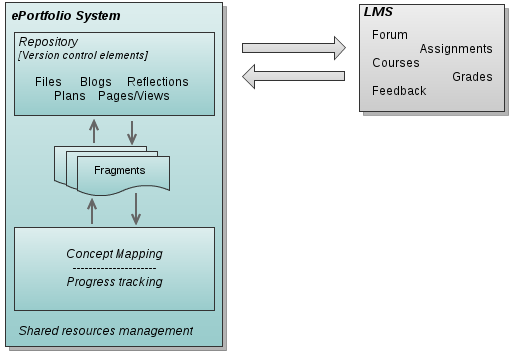
\includegraphics[width=0.9\textwidth]{CH6-F1-Architecture}
\caption{Environment architecture}
\label{fig:arch}
\end{figure}

In this project, the main implementations were carried out in the \ep~system
environment, Mahara. Due to cost vs benefit issues, features that involved LMS
environment, Moodle, were not considered for development. 

Benefit was analysed based on how high the interview participants had ranked
their requirements for \LLLs support. According to this, LMS aspects of system
support had not been identified as highly important in \LLLs context. 

The cost was measured by referring to the LMS developing communities that had
\ep~and LMS integration on their road-maps. For example, based on the issue
MDL-14591\footnote{\url{http://tracker.moodle.org/browse/MDL-14591} (Accessed
April 16, 2012)} on the Moodle LMS issue tracking system, it took one developer
from the development team, who probably had already been familiar with the
environment and its APIs, more than two years to develop an \ep~API that would
support single sign-on and enable simple data export/import functionality. To
date, this functionality still has a large number of unresolved issues and bugs
that require fixing (as can be seen from searching ``portfolio'' in Moodle Issue
Navigator\footnote{\url{http://tracker.moodle.org/secure/IssueNavigator.jspa}
(Accessed April 16, 2012)}).

As another example, based on discussions from ``Moodle and Elgg in Education''
group\footnote{\url{http://community.elgg.org/pg/groups/1057}
(Accessed April 16, 2012)} of Elgg community, more than 100 days were spent on development of a proprietary
plugin that would allow single sign-on and getting user statistics from Moodle
to Elgg.

Therefore, it can be concluded that investment into time and resources for the
development of the features that would allow integration between the systems
would exceed the benefit that would be gained from them by the users.

For these reasons, guidelines (G1 and G6) and features, that would have involved
modifications of Moodle LMS, were not realized by implementations and are not to
be discussed further in this chapter. However, for completeness, LMS is still
included in overall architecture as a system that supports formal learning in
universities.
 
Features identified through the interviews with the stakeholders were grouped
(based on groups described in Table \ref{tab:req}) and developed in the
following components and modules:

\begin{itemize}
  \item Version control -- for addressing the issues of guidance, facilitation
  and communication for \LLLsn;
  \item Artifacts' fragments extraction -- for better communication of specific
  part of \ep~and organizing learning materials;
  \item Concept mapping -- for linking abstract concepts to practical skills,
  managing \ep~knowledge, supporting reflection and developing awareness of
  personal learning achievements;
  \item Timeline based progress tracking -- for showcasing personal learning
  achievements and evaluation of progress towards learning goals;
  \item Shared resources management -- for addressing the issues of guidance
  and facilitation from non-institutional audiences, providing learners with
  better control over shared resources.
\end{itemize}

These components are discussed in detail further in this chapter.

Each component provided working functionality sufficient to demonstrate the
general concept. Some non-functional requirements, described in Chapter
\ref{cha:model}, were not taken into account during implementation as they did
not alter the prototype's essential functionality \citep{Robertson2006}. For
example, making fully visually appealing user interface was out of scope of these
implementations.

\section{Development Toolkit}

Using Mahara \ep~system as a base system defined technologies that were employed
in development phase. Development and prototype systems were installed on
LAMP\footnote{\url{http://en.wikipedia.org/wiki/LAMP_(software_bundle)}
(Accessed April 16, 2012)} software bundle for Linux which included Apache HTTP Server, MySQL database
server and PHP. These were the basic components for building a general purpose
web server.

Development environment consisted of the
Eclipse Platform with PHP Development
Tools\footnote{\url{http://eclipse.org/pdt} (Accessed April 16, 2012)}. A public
GitHub repository\footnote{\url{https://github.com/ybozhko/phd-mahara} (Accessed
April 16, 2012)} was used for code version control during development and
between the prototype iterations.

Following standards, libraries, and external packages were used during
implementation:

\begin{itemize}

\item HTML5\footnote{\url{http://www.w3.org/TR/html5/} (Accessed April 16,
2012)} + CSS\footnote{\url{http://www.w3.org/TR/CSS/} (Accessed April 16, 2012)}
-- standards combined with JavaScript used for drawing diagrams that represent concept maps, developing a
dynamic timeline and accessing fragments of media (audio/video);

\item jQuery\footnote{\url{http://jquery.com} (Accessed April 16, 2012)} -- a
JavaScript library that simplifies HTML document traversing, event handling, animating, and Ajax
interactions for rapid web development;

\item jQuery UI\footnote{\url{http://jqueryui.com} (Accessed April 16, 2012)} --
a JavaScript library built on top of the jQuery for development of highly interactive web applications;

\item jCrop v0.9.9\footnote{\url{http://deepliquid.com/content/Jcrop.html}
(Accessed April 16, 2012)} -- jQuery Image Cropping Plugin used in artifacts fragments (Section
\ref{sec:frag});

\item Graphic JavaScript Tree with
Layout\footnote{\url{http://www.codeproject.com/Articles/16192/Graphic-JavaScript-Tree-with-Layout}
(Accessed April 16, 2012)} -- a library that allows drawing dynamic concept maps. This library was
significantly modified to meet the needs of the project.
\end{itemize}

Prototype functionality was tested mainly in Google
Chrome\footnote{\url{http://www.google.com/chrome} (Accessed April 16, 2012)}
v14.0 and Mozilla Firefox\footnote{\url{http://www.firefox.com} (Accessed April
16, 2012)} v4.0 web browsers. Other web browsers (e.g. Microsoft Internet
Explorer\footnote{\url{http://www.microsoft.com} (Accessed April 16, 2012)})
that did not provide native support for HTML5 elements such as Canvas, required for concept map layout, and
embedded video/audio, used in artifact's fragments, were not used in testing.

\section{Implementations}

Components added to the standard Mahara \ep~installation were expected to
address the requirements developed by the stakeholders and derived from the
literature review. In most cases, the suggestions from stakeholders, when they
provided their own vision of what kind of features could have been implemented
to solve particular problems, were used during development. In other cases,
where the stakeholders could not propose any suitable solution, it was necessary
to refer to other domains and analyse solutions to similar problems. In this
case, most suitable, as well as feasible for development, approach was adopted.

Table \ref{tab:implement} matches implemented components to the guidelines they
support and the requested features. Guidelines and feature identifiers used in
this table were described in Sections \ref{sec:needs} and \ref{sec:elicit},
respectively.

\begin{table}[htb]
  \setlength{\abovecaptionskip}{0pt}
  \caption{Matrix of implemented \ep~system components}
  \begin{center} \small
    \begin{tabular}{| c || p{2cm} | p{2cm} | p{2cm} | p{2cm} | p{2cm} |}
    \hline
     \multicolumn{1}{|c||}{} &
     \multicolumn{5}{c|}{\textbf{Implemented components}} \\ \cline{2-6}
     \textbf{Guidelines} & 
     \textit{Version \newline control \newline Section \ref{sec:version}} & 
     \textit{Concept mapping \newline Section \ref{sec:mapping}} & 
     \textit{Artifacts' fragments \newline Section \ref{sec:frag}} & 
     \textit{Progress tracking \newline Section \ref{sec:timeline}} & 
     \textit{Managing \newline sharing \newline Section \ref{sec:sharing}} \\
     \hline \hline
     \rowcolor[gray]{.8} G1 & & & & & \\ \hline
     G2 & F7.3 & & & F3.1 & F6.3\\ \hline
     G3 & F7.3 & & & & F6.3 \\ \hline
     G4 & & F1.1, F1.2 & F1.2 & & \\ \hline
     G5 & F3.2, F3.3, \newline F3.4 & & F3.4 & & F3.5, F3.6 \\ \hline
     \rowcolor[gray]{.8} G6 & & & & & \\ \hline
     G7 & & F2.1 & & F2.1, F2.2, \newline F2.3 & \\ \hline
     G8 & & F5.1, F5.2, \newline F5.3, F5.4, \newline F5.5, F5.6 & & & \\ \hline
     G9 & & F6.1 & F1.3 & F2.4, F2.5 & \\ \hline
    \end{tabular}
  \end{center}
  \label{tab:implement}
\end{table}

\FloatBarrier

Table \ref{tab:implement} also shows that implementations are covering at least
partially each of the guidelines. Complete lists of the requirements for each
component in the form of user stories are described in the relevant sections of
Appendix \ref{app:specification}. Detailed screenshots of the interface can be
found in Appendix \ref{cha:appscreen}.

\subsection{Version Control Elements}
\label{sec:version}

Version control adopted in this prototype resembles functionality of standard
revision control systems (such as Git\footnote{\url{http://git-scm.com}
(Accessed April 16, 2012)},
Subversion\footnote{\url{http://subversion.apache.org} (Accessed April 16,
2012)}, or Concurrent Versions
System\footnote{\url{http://savannah.nongnu.org/projects/cvs} (Accessed April
16, 2012)}) that allow management of changes in the documents, source code, and
other types information stored in files.

Creating and keeping versions of the shareable resources was suggested by the
stakeholders as a way of communicating changes made to the \ep~items and
responding to the comments and feedback. According to the systems review in
Chapter \ref{cha:systudy}, conventional functionality of the \ep~systems does not
support multiple versions of repository items or web pages making it difficult
to track changes being made. Normally, when learners get feedback on the shared
part of their \ep, they would just apply changes according to this feedback
making it nearly impossible for others to compare what was actually altered.
This results in a mismatch because feedback still refers to the old version of
shared \ep~while content is already renewed. Being able to take snapshots of
various \ep~parts is a simple solution requested by the stakeholders to address
this problem.

This feature was easy to fit into the system and straightforward to implement.
As every record in \ep~has its own time-stamp, all that was required was to
create a new copy of the current record, allow users to make changes and,
after changes are saved, present the new record to users in a way that would
allow tracing back to the previous versions.

A simple revision control implemented in the prototype supported \textit{parent}
$\to$ \textit{child} relationship between versions (Figure \ref{fig:version}),
but did not support versions branching as in complex revision control systems.
This made it possible to bring work with versions to intuitive level for less
computer-savvy learners.

\begin{figure}[htb]
\centering
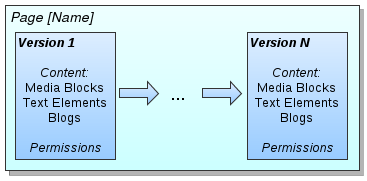
\includegraphics[width=0.7\textwidth]{CH6-F2-Version}
\caption{Page version control}
\label{fig:version}
\end{figure}

Creating a new version of an item is triggered by users on demand and is not
done automatically every time user alters or saves the item. This allows users to
control what they want to save and when.

As can be seen from the requirements in Table \ref{tab:req1}, this feature was
implemented for the \ep~pages. It was considered sufficient to demonstrate the
general concept as \ep~pages could be shared with others, and experience of
using this feature can be easily transferred to other shareable resources.

The component does not perform an automated difference analysis between versions
because pages can incorporate both textual and block elements that would make it
technically difficult and time consuming to implement this kind of analysis.
Therefore, analysing the difference between versions was left for users.
 
Adopting version control elements in \ep~system was expected to provide support
for communication and feedback-response cycle between students and lecturers, as
well as between students and audience outside of institutional environment.

\subsection{Concept Mapping Module}
\label{sec:mapping}
Addressing the challenges of \ep~knowledge management\footnote{In this thesis,
the \ep~knowledge management is referred to in terms of creating knowledge,
sharing it, managing and organizing it in \ep~space.} and development of
graduate attributes was a complex problem which required a creative approach and
no clearly suggested solution from the stakeholders. While looking at the other
areas for potential solution, it was discovered that qualitative data analysis
and knowledge visualization using concept mapping tool have properties suitable
for \ep~domain. Like \ep~work, qualitative data analysis is characterised by
rich data sets, opening the possibility of borrowing well established
techniques. Concept maps had potential as a supporting tool for organizing these
data sets into concepts and visualising them in a way that could be understood
by relevant audiences.

This section describes how bringing these two techniques together helped to
develop a solution for the problems outlined earlier.

\subsubsection{Parallels to qualitative research}

An \ep~can be called a container whose content needs to be organized, with
students not always knowing which items to select and where the items they put
in their \ep~should go. Students start their \ep~work by collecting \textit{raw}
data available from formal learning and outside activities and transforming it
into information that they decide to put into their \ep. After working with and
reflecting on this information students arrive at knowledge. However, sometimes
there is just too much data for students to cope with efficiently as they might
be initially lacking organizing skills. In this case, an \ep~system could
provide supporting solutions to help students manage their data.

A parallel with qualitative data analysis can be drawn here where researchers
either develop new theories from data, moving from specific observations to
general concepts and theories (inductive approach), or they try to check if
their data map against the theories that are already known and understood
(deductive approach) \citep{Strauss2008,Patton2002}. An assumption here is that
analyzing one's own learning process takes similar steps as qualitative data
analysis: small bits, specific data that learners are collecting, contribute to
the bigger picture of knowledge development. 

The difference is that the learner developing their \ep~is not aware of the
existing theories yet. These theories are the concept structures that exist in
the understanding of society, institution and employers. However, these must be
eventually understood and \textit{made their own} by the learner. Like the
qualitative researcher, the learner needs to immerse themselves in their data
and to come to an understanding of the kind of material they should be
collecting in their \ep~and the concepts that express their learning goals. They
need to find (and to a certain degree construct by exposing themselves to
learning opportunities) evidence in their data to show that they conform to
these concepts.

In qualitative research, a number of techniques are available to the researcher
in managing, analyzing and interpreting their data, such as coding, grouping,
generating categories and themes, rearranging and sorting \citep{Marshall2010}.
To support these techniques, specialized qualitative data analysis software
(QDAS), like
NVivo\footnote{\url{http://www.qsrinternational.com/products_nvivo.aspx}
(Accessed April 16, 2012)} and MAXQDA\footnote{\url{http://www.maxqda.com}
(Accessed April 16, 2012)}, has been developed which largely allows coding,
linking and mapping unstructured information. Although, QDAS could provide
students with necessary functionality for data analysis, it cannot substitute
the role of an \ep~system in the learning process. Reasons for that are outlined
in Table \ref{tab:qdas}.

\begin{table}[htb]
  \setlength{\abovecaptionskip}{0pt}
  \caption{Conceptual difference between QDAS and an \ep~system}
  \begin{center}
    \begin{tabular}{| p{6.5cm} | p{6.5cm} |}
    \hline
     \multicolumn{1}{|c|}{\textbf{QDAS}} &
     \multicolumn{1}{c|}{\textbf{An \ep~system}} \\
     \hline
     Do not share the analysis data & Showcase parts of the \ep~content to
     others \\ \hline 
     Only intermediate steps/data are contained, the research findings are
     written and communicated outside the system & Reflections, pages and data
     are apart of the \ep \\ \hline 
     Produce a report as an end point of the research  & Does not have an end
     point; data is constantly evolving; old concepts are changing and new are
     emerging with changing understanding of these concepts \\ \hline
    \end{tabular}
  \end{center}
  \label{tab:qdas}
\end{table}

However, the strength of QDAS is in how it allows to work closely with data.
Researchers \textit{label} data with codes, not just in order to connect these
labels later, but as an opportunity to \textit{dive} into their data by
re-reading, listening or watching it over and over again. This strength is
important for students as they need to revisit their material as their
understanding of concepts grows.

Currently, the majority of \ep~systems allow tagging their content with
user-defined tags. However, according to the results of interviews with
students, tagging does not provide necessary meaning to the \ep~data,
cannot show relations between concepts and does not allow building a flexible
structure. To address this problem, concept mapping was introduced into
\ep~environment to help students to be able use the same techniques available in
qualitative data analysis to manage unstructured data and develop learning
concepts in their \ep.

\subsubsection{Concept maps}

\citet{Mcaleese1998} formally defines a concept map as a directed acyclic graph
that consists of a set of Concept Labels and a non-empty set of Relationships
between Concepts. Putting it simply, concept maps are graphical representation
of the hierarchy of knowledge concepts and connections between them
\citep{Novak2008}.

Concept maps fit well with the qualitative data analysis techniques, outlined in
the previous section, as they are dynamic, process-oriented and give learners an
opportunity to engage in the learning process \citep{Mcaleese1998} which is
important for \LLLs \citep{Schuetze2006,Divjak2004}. Maps are created over time
by the learner who is engaged in a process of reflection, collecting and
selecting appropriate examples of their work. With concept maps, learners can
interpret their personal knowledge and map this knowledge and individual
examples against the existing theories. The hierarchical nature of the concept
map allows for organizing concepts from the high level abstract concept to the
more specific concepts. This property can be used by students for managing and
structuring data in their \ep s. 

In addition to the conclusions drawing from comparison with qualitative data
analysis, support for utilizing concept maps also comes from the literature.
While describing future directions for \ep~technology, Cambridge
\citeyearpar{Cambridge2010} suggested that visualization in the form of concept
maps could be a potential way of generating reflections.

QDAS already offers tools similar to concept maps in form of textual hierarchies
of nodes/terms/labels/concepts or as diagrams that show relations between
labels. Adding concept maps functionality to an \ep~system might make it
possible to borrow well established techniques of qualitative data analysis and
help students, who are analyzing their learning, to formally do what QDAS
already does informally. 

Concept maps have been already successfully used to in education to communicate
complex ideas, assess understanding of learning objectives, elicit knowledge and
provide conceptual frame for learning \citep{Novak2010}. A complete review of
the concept maps is beyond the scope of this thesis. For detailed examples and
evaluation of effectiveness of this tool refer to The Institute for Human and
Machine Cognition research group report \citep{Canas2003}.

\subsubsection{Component implementation}

The component (Figure \ref{fig:mapping}), presented in this section, adopts the
idea of concept maps in terms of developing or understanding concepts and
relations between them. Following qualitative data analysis techniques, students
create their own codes for the concepts which later form a concept map. Students
can also be provided with a map structure predefined by universities as a set of
Graduate Attributes in form of abstract concepts. Going through the program of
study, students can learn to understand these concepts and recognize the
valuable examples of their work in the learning process.

\begin{figure}[htb]
\centering
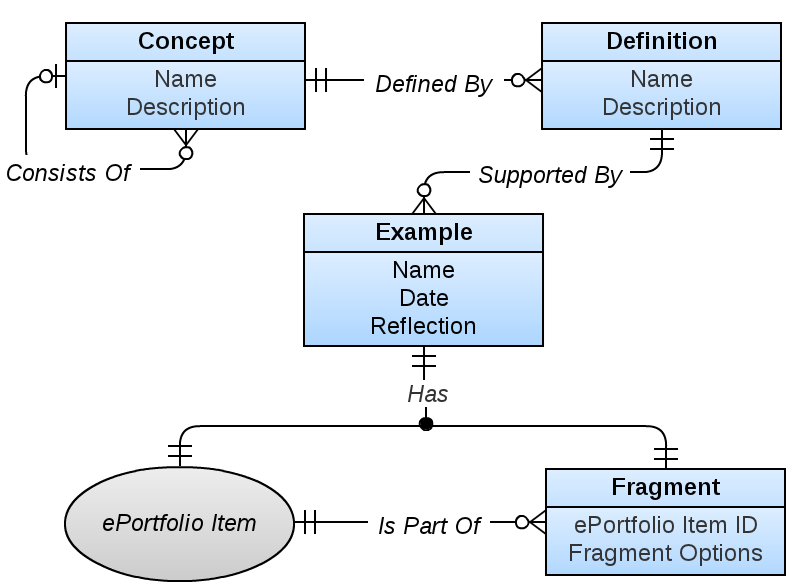
\includegraphics[width=0.7\textwidth]{CH6-F3-Mapping}
\caption{ER diagram of the concept mapping elements}
\label{fig:mapping}
\end{figure}

Using a \textit{tree} is considered to be the commonly used and natural way
of visualizing hierarchical data \citep{Gorg2007,Holten2006}. Trees are more
visually appealing, easier to master, and since trees are hierarchical, they are
better understood by many people. According to \citet{LeGrand2006}, they are
also easier to interpret than graphs. Therefore, instead of implementing a
complete directed acyclic graph structure, as described in the previous section,
concept mapping in this component was simplified to a tree-like structure and
did not provide cross-linking between the concepts.

Each map starts with an abstract core or key concept followed by optional
supporting sub-concepts. Hierarchy of the concepts can go as far as required by
learners starting from highly abstract concepts and going to very specific ones.
As shown on Figure \ref{fig:mapping}, students can provide definitions for the
concepts, which gives them descriptions from learners' point of view. As it was
noticed from the interviews with the stakeholders, often students do not
understand the meaning of the concepts offered by the university in the graduate
profiles or attributes. In this case, being able to provide own definitions to
the concepts, might help learners to express their own understanding and
communicate it to others.

Examples chosen by students for the concepts and definitions represent their
personal experiences and achievements. These examples are the fragments of
items, or entire items, from the \ep~repository. A detailed description of this
feature can be found in Section \ref{sec:frag}.

\begin{figure}[htb]
\centering
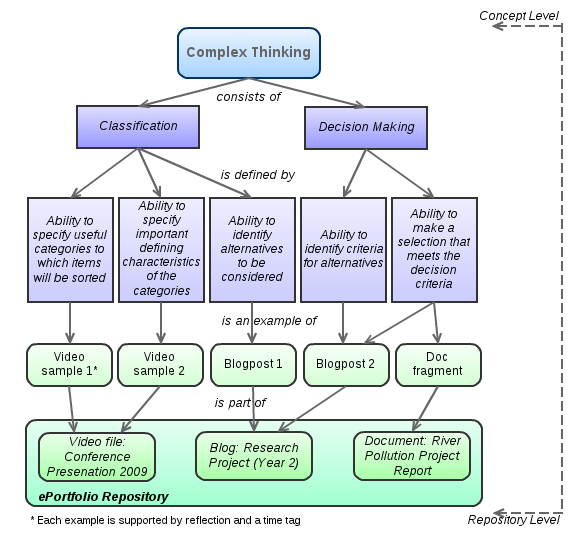
\includegraphics[height=0.5\textheight]{CH6-F4-Map-Example}
\caption{Concept mapping framework applied to the example}
\label{fig:mapex} 
\end{figure}

An \ep~concepts structure can be represented as shown in Figure \ref{fig:mapex}.
Data for the example was taken from the examples offered by \citet{Marzano1993}
on how to assess \LLLs standards.

Due to the dynamic nature of learning process, this kind of structure might
never be complete. It is constantly changing as students deepen their
understanding and potentially find more suitable evidence to underpin their
development.

\FloatBarrier

The expectations are that this approach would allow students to:
\begin{itemize}
  \setlength{\parskip}{0pt}
  \setlength{\parsep}{0pt}
  \setlength{\itemsep}{2pt}
  \item Manage and structure large amounts of information in their \ep:
  students will be able to organize and navigate through the information, find
  relations between the content and the concepts and see the data in their
  \ep~from various perspectives: from an item belonging to different
  structures; from a concept containing multiple evidences; and from items and
  concepts attached to a timeline (Section \ref{sec:timeline});

\item Share their progress/development map with others for feedback or
evaluation: students will be able to create specific structures for various
purposes to show to the audience specific parts of their \ep~(for example,
share with a potential employer communication and writing skills developed over
the last year at university);

\item Access and address institutional graduate attributes: by providing
students with a concept map of the graduate attributes (maybe even already
supported by the institutional definitions), universities would be able to
help students to understand the skills requirements of their study area and look
at their study program from the \LLLs perspective;

\item Develop a flexible structure for self-directed learning: students are
provided with all operations necessary to make their structures flexible such as
creating new concepts, removing or merging existing ones, creating links between
structure fragments and taking snippets of \ep~items as examples (Section
\ref{sec:frag});

\item Facilitate setting up learning/development goals and expressing students
visions of their knowledge: constructing their own concepts and definitions
might encourage students to think of what skills are important to them, how they
understand these skills and how it links to their learning outcomes.
\end{itemize}


\subsection{Artifacts' Fragments Extraction}
\label{sec:frag}

Artifact's fragments extraction was developed as a part of the concept mapping
module. This feature allows selecting \ep~artifact's fragments and using
them as example in definitions of the concepts described in the previous
section.

The idea behind this feature was to allow students to share specific parts of
\ep~artifacts linked to the conceptual level of their learning. Because
extracting a fragment is a part of creating an example to the concepts, each
fragment has to be supported by the student's reflection. Reflection should
explain what is so special about this example, or how it addresses some specific
concept which it refers to. It is expected to help students understand that
their \ep~space is not a place for \textit{dumping} all possible items. Each
element of an \ep~is an important example of their personal and professional
development carefully selected to showcase learning progress.

When learners create a fragment as a part of an example, they can link it
directly to the concepts that already exist in their \ep. In case learners do
not know where this example belongs to in the hierarchy of concepts, they can
leave it as a free fragment and use later.

To demonstrate this feature, the following artifact fragments were implemented:

\begin{itemize}
  \item Image: JPEG, PNG, GIF -- by selecting of a part of an image;
  \item Video: OGV, MP4, 3GP, WEBM -- by specifying start and end time of a
  fragment;
  \item Text: TXT -- by selecting a text fragment;
  \item Blog -- by selecting one or more blogposts;
  \item Bookmark: URL of the resources on the Internet -- no selection is
  required.
\end{itemize} 

Figure \ref{fig:frag} shows the way of extracting fragments for various
\ep~artifacts.

\begin{figure}[h!]
\centering
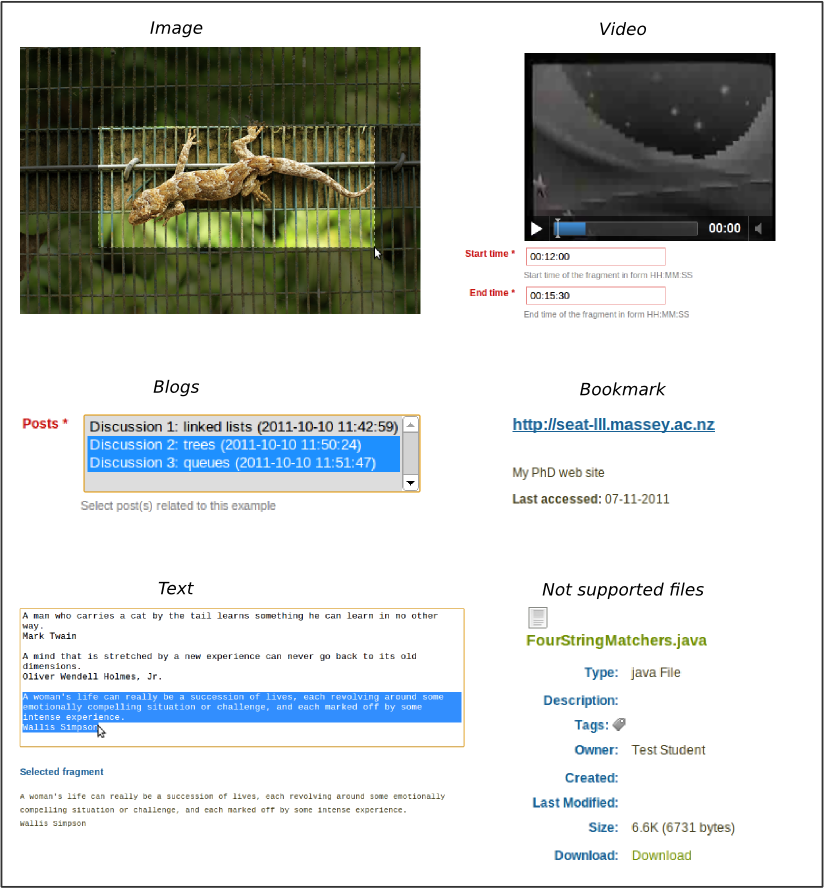
\includegraphics[width=0.99\textwidth]{CH6-F5-Fragments}
\caption{Artifact's fragment extraction}
\label{fig:frag}
\end{figure}

\FloatBarrier

At this stage, fragments of textual files support only TXT files because
popular, but proprietary formats as PDF or DOC do not allow selecting fragments.
Although it is possible to access specific fragments of PDF documents through
fragment identifiers, it is not possible to extract the fragment and restrain
access to this fragment only.

Files that do not support fragments extraction allow attaching an entire
artifact for download. Each extracted fragment can be as well accompanied with a
link to the item in case learners would want to allow its download.

Using fragments of artifacts can be useful for a number of reasons:
\begin{itemize}
  \item it allows to draw attention to a specific part of artifacts (like part
  of a picture, or fragment of a video);
  \item it allows the presentation of different parts of artifacts to different
  audiences;
  \item it helps to avoid files duplication;
  \item it saves user's time that otherwise would be spent on cropping images,
  videos, or textual files;
  \item it can help to solve some ethics issues (for example, students studying
  to become teachers are not allowed to show the faces of children they teach at
  schools, but they still have to demonstrate their competencies of teaching).
\end{itemize}

From the perspective of this component evolving Media Fragments 1.0
specification \citep{MediaGroup2011} becomes very useful as it describes the
ways of extracting temporal and spatial media fragments using Uniform Resource
Identifiers (URI). Once it is finished (as planned for December 2011 -- January
2012), this specification could be adopted in the \ep~system for improved
fragments description and extraction.

\subsection{Learning Progress Tracking}
\label{sec:timeline}

Timeline representation of learning progress was developed in conjunction with
concept mapping component. It is used to present the data from the concept map
in chronological order.

Timelines are used in various areas, such as education, history, natural
sciences, software development and project management, for presenting and often
visualizing a progression of related events. This valuable property of a
timeline to show progression was used in the prototype development to bring a
sense of change over time to the learners analysing their personal or professional
development.

Timelines in the prototype are generated automatically and do not require
user's input. Each example described in the previous section is accompanied with
a \textit{time tags} whether is it taken from the properties of the artifact as
creation date or added as a customary selected date. These time tags of the
examples allow any concept map to be transformed into a timeline, as shown on
Figure \ref{fig:timeline}. Each entry on the timeline is an example from the
concept maps.

\begin{figure}[htb]
\centering 
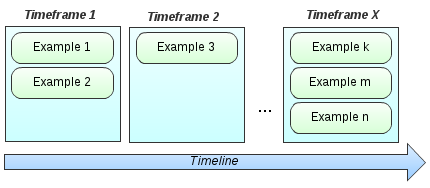
\includegraphics[width=0.75\textwidth]{CH6-F6-Timeline}
\caption{Timeline structure}
\label{fig:timeline}
\end{figure}

Standard representation of the timeline uses a linear time scale available in
two options, i.e., month and year. In addition to the standard representation,
users can create their own time scales with the custom time frames (e.g., BA
year 1, BA year 2). In custom time frames, users need to specify start and end
date of the frame. Examples are then grouped and visualised under a specific
time frame based on their time tags. 

Users can navigate through any part of the timeline by clicking on the bar
labeled with time frames. Clicking on the entry brings up a window with the
details of the example: title, reflection and concept it belongs to.

Information on the timeline can be filtered based on the concepts hierarchy of
the map. This can be used to see the progress towards development of some
specific concept(s), changes in feedback and improvements of the examples.

Adoption of this component is expected to provide support for tracking personal
progress in various areas and aspects. Generating timelines could add a temporal
dimension to students progress analysis: they would be able to see how their
skills evidence changed with time, how feedback received from the others
reflects their growing understanding, what achievements they have made and what
concepts require more input. It could also help to showcase the progress for
evaluation or share it with others for feedback purpose.

\subsection{Shared Resources Management}
\label{sec:sharing}

To be able to share the parts of \ep~in a way required by the stakeholders was
another important aspect of \LLLs support that needed improvements. As was shown
in the previous chapters, current \ep~systems already provide extensive list of
sharing options: by email, secret URL, temporary accounts, etc. However,
managing shared resources was missing from the features provided by these systems.

The following improvements were implemented in this area to provide a better
control over shared resources:

\begin{itemize}
  \item Saving sharing/access history: every time a page or a concept map is
  shared with others a record is created in the user access log. This allows the
  user to review when a part of \ep~was shared and with whom; 
  \item Easy re-share through access history: Saving access history made it
  possible to re-share resources with the same audience once their access
  expires;
  \item Notifications on access expiry for system users and resources shared by
  email: if set up by a learner, when access to the shared resources is close to
  the expiry date, the system sends notification to people on the access list;
  \item Control over level of feedback provided: bringing concept mapping with
  its hierarchy of concepts and examples into \ep, opened opportunity to give
  learners control over level of feedback they expect to get. In concept maps,
  learners can choose what kind of feedback they want, whether it is feedback on
  overall map structure, individual examples or a group of examples related to a
  concept. From lecturers' perspective, it allows them to attach their feedback
  to the elements of a concept map which means that they can focus on specific
  aspects as well as on the general picture.
\end{itemize}

Better control over shared resources has potential to bring more confidence to
learners, support dialog between interested parties, improve quality of
feedback, and facilitate its provision in a timely manner.

\section{Prototype Iterations and User Tests}
 
Before formal evaluation was undertaken, implemented functionality had been
reviewed by users. Overall, despite time and resources constraints of the
project two prototype iterations were possible. Each iteration produced a
workable version of the implemented features. At the end of each iteration, the
functional prototype was presented to a student and a lecturer selected from the
participants of the requirements elicitation phase who had agreed to continue
their participation in this research.

Each feedback session included up to an hour demonstration and discussion of the
implemented functionality. Users were encouraged to give their ideas about
additional improvements and provide their thoughts on possible drawbacks of
presented implementations.

Feedback between iterations was very useful as it facilitated further discussion
with the stakeholders and helped to get more information on potential
improvements. Users were generally satisfied with the improvements and made
largely positive comments. However, several issues were noticed. Most notably,
users mentioned that they would have difficulties using the system on their
own without comprehensive instructions. Some features not common for web
interfaces, like right-click context menu in concept mapping, might confuse
novice users. It was decided that starting tips on the web-pages could be an
additional help to the beginners who are not familiar with the system.

All discovered issues were addressed in the later versions of the prototype
in preparation for the formal evaluation stage.

\section{Summary}

This chapter presented design and implementation of additions and improvements
of the \ep~system based on the needs of the stakeholders and \LLLs success
guidelines discovered in the literature. A set of features was introduced to
the standard \ep~installation with the aim to address various aspects of \LLLs
support in universities. These features are expected to support understanding,
development an showcasing of \LLLs skills, learning progress tracking,
management of \ep~content and knowledge, communication between students and
lecturers, and better control over access to the \ep~resources.

From this stage, to understand whether new implementations meet the needs of
the stakeholders, a formal evaluation has to be undertaken. The next chapter
looks at the improved \ep~system prototype from the perspective of lecturers
and students with various levels of experience.
